\chapter{Results}
\label{sec:results}

\section{Baseline Performance}
\label{sec:results-baseline}

\begin{figure}[htbp]
\centering
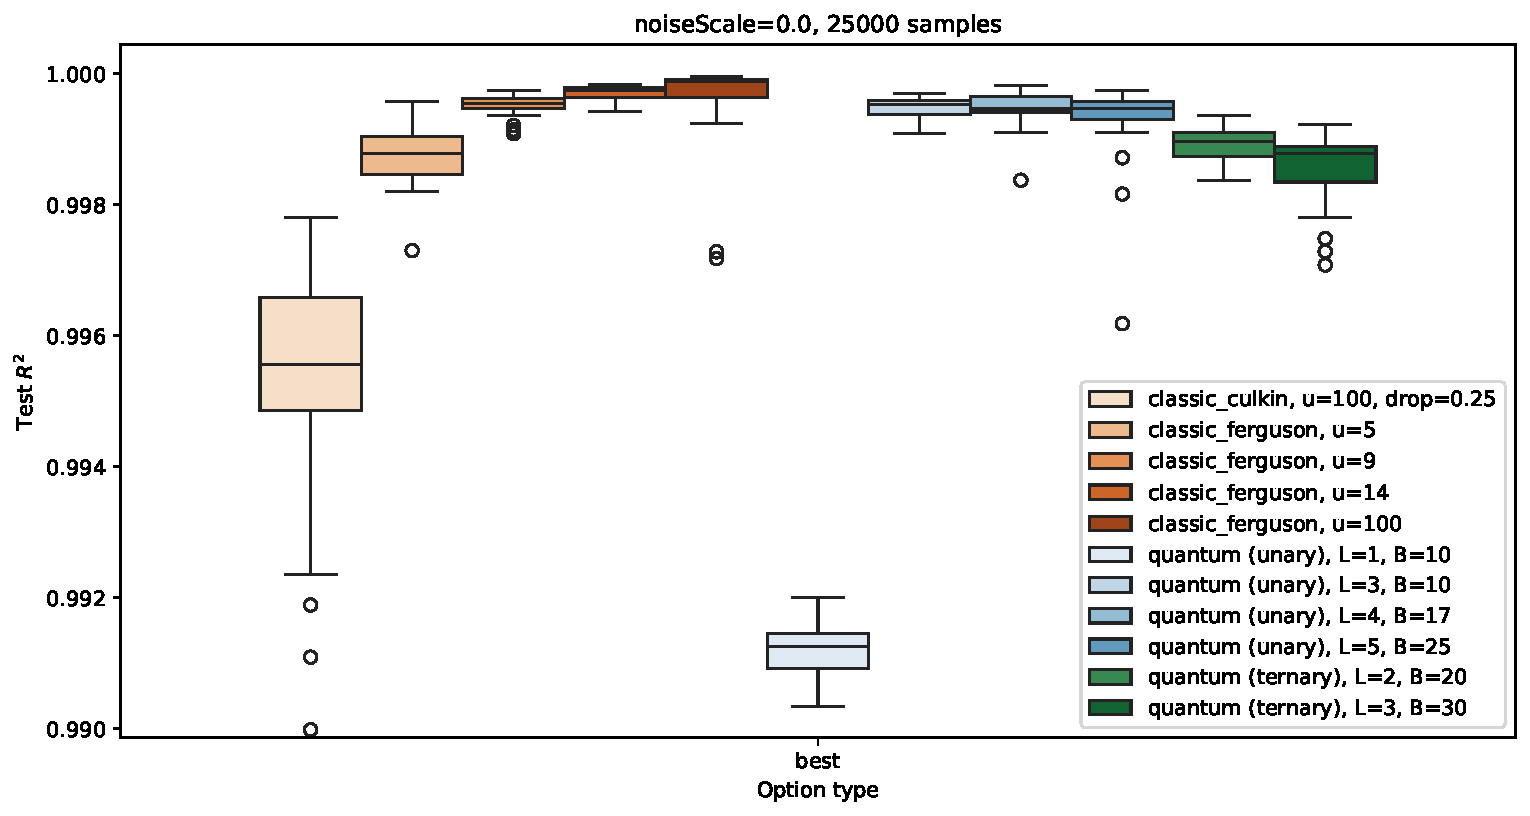
\includegraphics[width=\linewidth]{pictures/boxplot_optiontypes_nS0_nsp25k_best.pdf}
\caption{
Distribution of test-$R^2$ values across 30 seeds for Best-of basket options
in the baseline scenario (full training dataset, no artificial noise).
}
\label{fig:baseline_best}
\end{figure}

Figure~\ref{fig:baseline_best} shows the results in the baseline scenario
for Best-of options. All models achieve very high test-$R^2$ values,
indicating that the underlying pricing structure of the options can be
well approximated by the considered model architectures.

For the classical Ferguson models, a clear relationship between model
size and performance can be observed. The median test-$R^2$ increases
from $0.9988$ ($u=5$) to $0.9995$ ($u=9$), $0.9997$ ($u=14$), and
finally $0.9999$ for the largest model ($u=100$).

Despite a comparable model size, the Culkin model achieves lower
accuracy (median $R^2 = 0.9956$),
which is likely due to the use of dropout ($p=0.25$), which is not
necessary in the noise-free baseline scenario.

For the quantum models, a larger model size does not necessarily lead
to better performance. While the performance improves substantially
from the smallest model ($L=1$, median $R^2 = 0.9912$) to larger
models, only minor differences are observed afterwards. The unary
encoding models with $L=3$, $L=4$, and $L=5$ reach nearly identical
median values of approximately $0.9995$.

When comparing the encoding strategies, unary models tend to perform
slightly better than ternary models. For example, the unary model
($L=4$, $B=17$) achieves a median test-$R^2$ of $0.99946$, whereas
the ternary model with a comparable frequency spectrum ($L=2$,
$B=20$) achieves a median of $0.99897$.

For this reason, ternary models are not considered further in the
following experiments. In addition, one of the classical Ferguson
models is omitted in the subsequent experiments for improved
readability.

\begin{figure}[htbp]
\centering
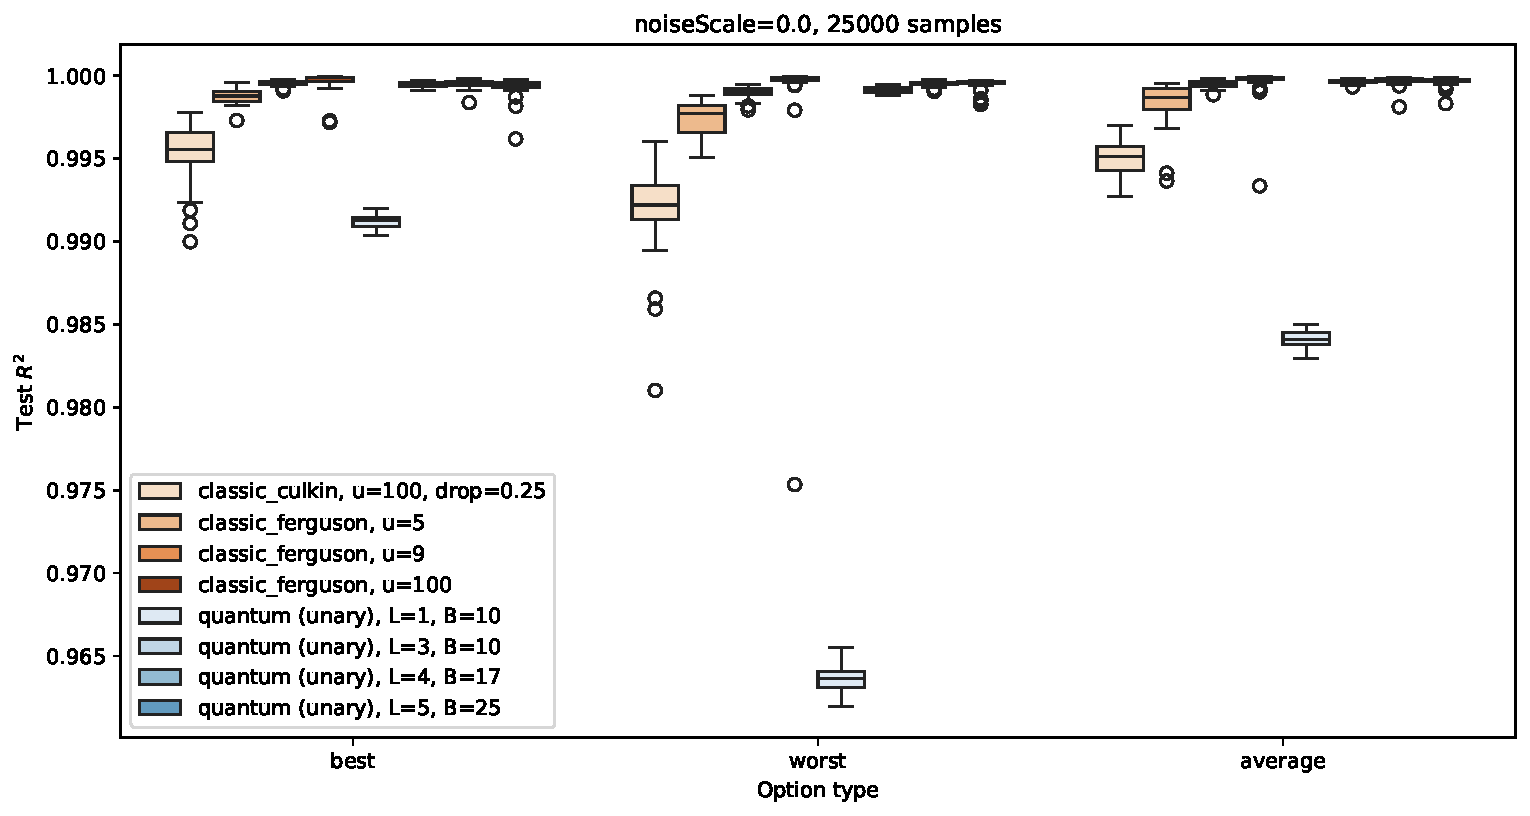
\includegraphics[width=\linewidth]{pictures/boxplot_optiontypes_nS0_nsp25k.pdf}
\caption{
Distribution of test-$R^2$ values across 30 seeds for Worst-of,
Best-of, and Average basket options in the baseline scenario
(full training dataset, no artificial noise).
}
\label{fig:baseline}
\end{figure}

Figure~\ref{fig:baseline} shows the distribution of test-$R^2$ values
for Best-of, Worst-of, and Average basket options.

For Average basket options, the results are very similar to those of
Best-of options, with median values typically exceeding $0.9995$.
For example, the Ferguson model with $u=9$ achieves a median test-$R^2$
of $0.99946$, while the largest model ($u=100$) reaches $0.99983$.
The larger quantum models also achieve high values, such as
$0.99965$ ($L=3$) and $0.99972$ ($L=4$).

The Worst-of payoff, however, represents the most challenging
approximation task. Here, the test-$R^2$ values are slightly lower
overall, particularly for the smallest quantum model ($L=1$,
median $R^2 = 0.9637$). With increasing model capacity, however,
performance improves significantly. The unary models with $L=3$,
$L=4$, and $L=5$ reach median values between approximately
$0.99906$ and $0.99958$. A similar trend can also be observed for
the classical models, where the median increases from $0.99907$
($u=9$) to $0.99986$ ($u=100$).

The slightly lower performance for the Worst-of payoff may be due to
the fact that it is not only bounded below by $0$, but also bounded
above by the value of the respective other asset. This additional
structure may complicate the approximation and lead to slightly
lower test-$R^2$ values.

For additional qualitative insights,
Figure~\ref{fig:qualitative-baseline} shows the relationship between
target values and model predictions for a representative seed in the
Worst-of scenario.

\begin{figure}[htbp]
\centering
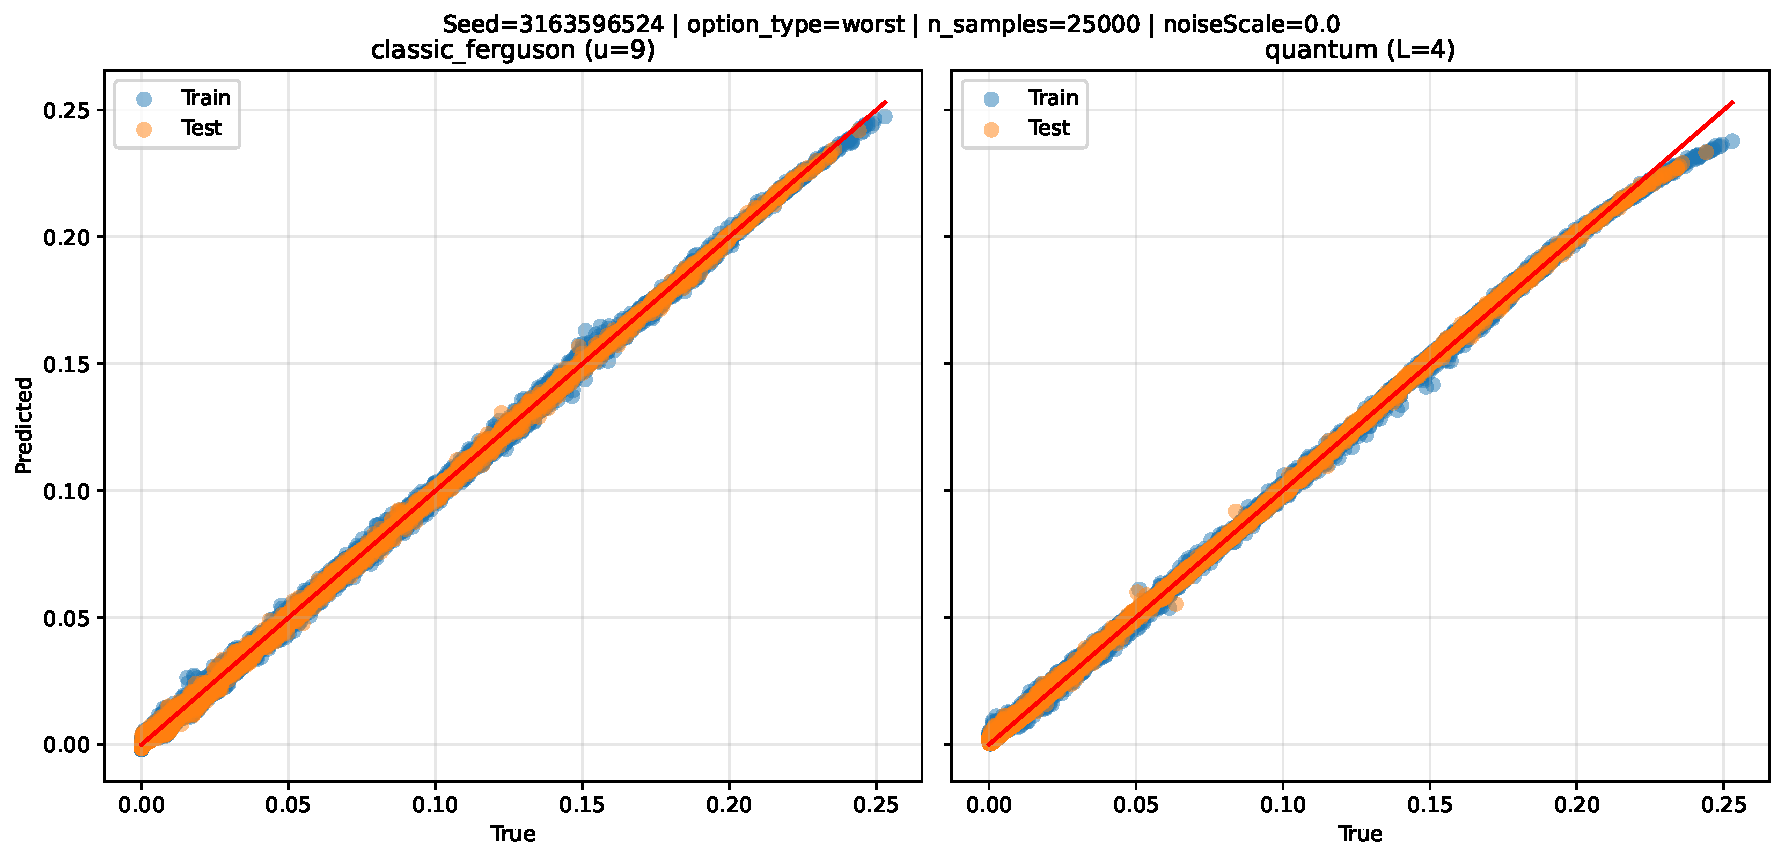
\includegraphics[width=\linewidth]{pictures/scatter_baseline.pdf}
\caption{
Predictions versus target values for a representative seed in the
baseline scenario (Worst-of, $N=25000$, $\alpha=0$). Left: Ferguson
($u=9$), right: VQC ($L=4$). The red diagonal indicates perfect
prediction.
}
\label{fig:qualitative-baseline}
\end{figure}

Both models show a strong concentration along the 45° diagonal,
which visually confirms the high test-$R^2$ values. No systematic
differences between training and test data are observable.

However, in the right panel it can be seen that the VQC tends to
systematically underestimate larger target values ($\hat{y} < y$).
The deviations increase with increasing target values, and the
point cloud shows a slightly curved structure relative to the
diagonal in the upper value range.

For further analysis, Figure~\ref{fig:error-analysis} shows the
signed error
\(
e = y - \hat{y}
\)
on the test data.

\begin{figure}[htbp]
\centering
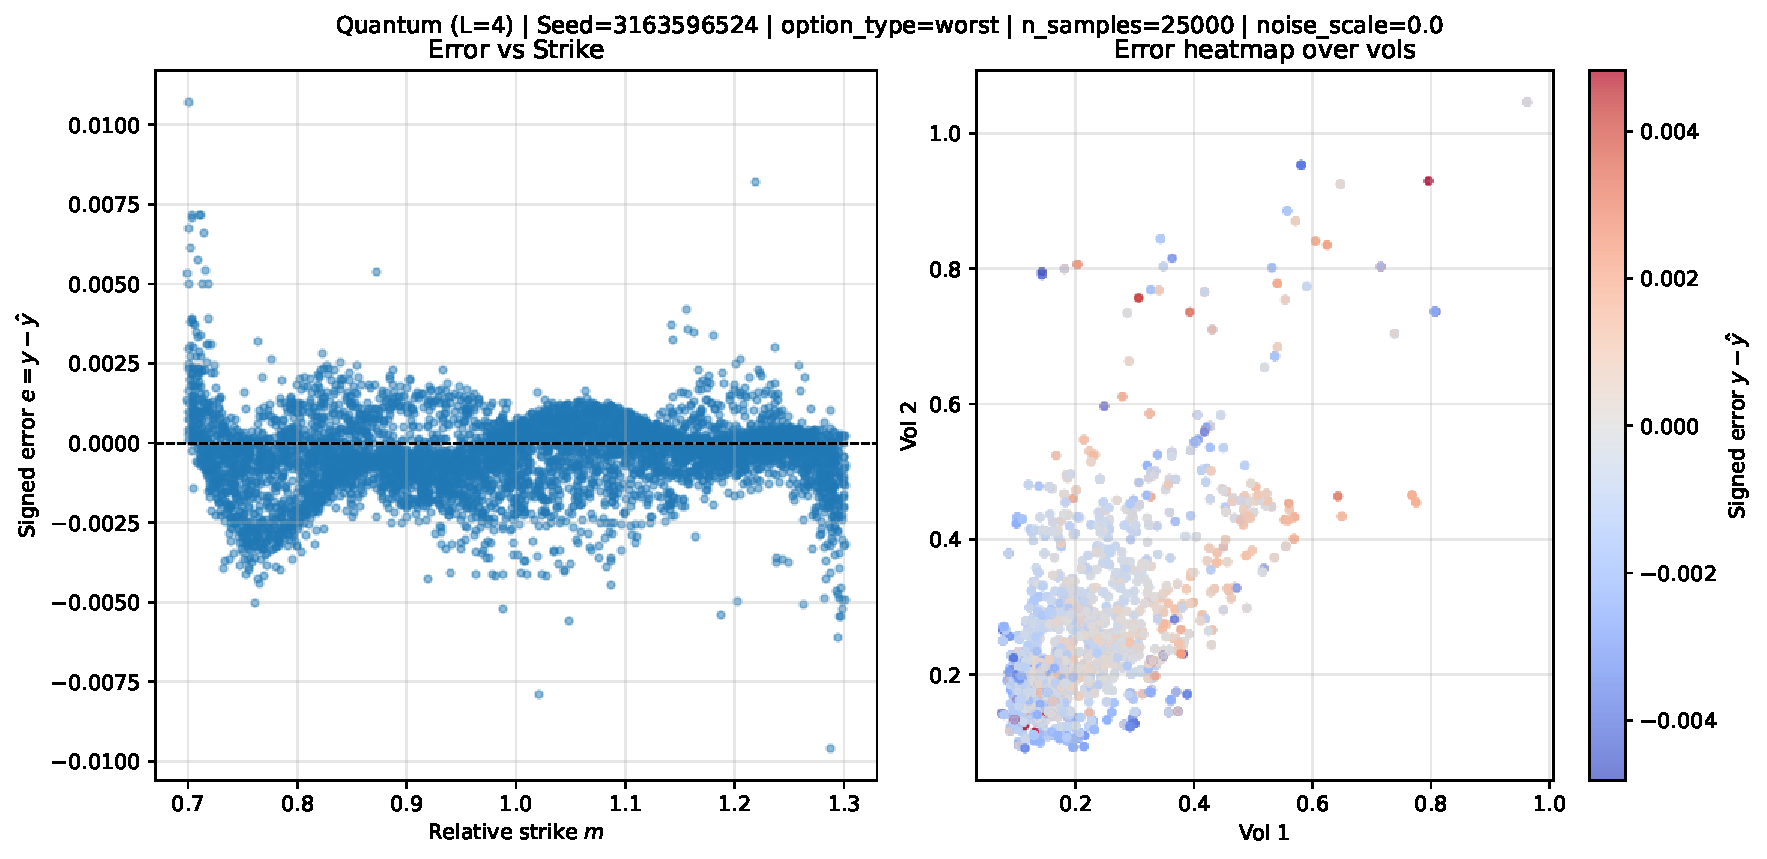
\includegraphics[width=\linewidth]{pictures/error_analysis_baseline.pdf}
\caption{
Error analysis on the test data for the same seed in the baseline
scenario. Left: error as a function of relative strike $m$. Right:
color-coded error across the two volatility dimensions.
}
\label{fig:error-analysis}
\end{figure}

Stronger positive errors occur particularly for low relative strikes
($m \approx 0.7$), corresponding to a systematic underestimation of
high option prices in this moneyness region. Since lower strikes lead
to higher option prices, this region corresponds to the upper range
of target values, which is consistent with the previously observed
underestimation of high prices.

In the projection onto the two volatility dimensions, however,
no clear spatial pattern can be identified. The errors therefore
appear to be primarily related to the strike level or the function
value itself, while no dominant relationship with specific volatility
combinations can be observed.

\section{Impact of Training Dataset Size}
\label{sec:results-samples}

\begin{figure}[htbp]
\centering
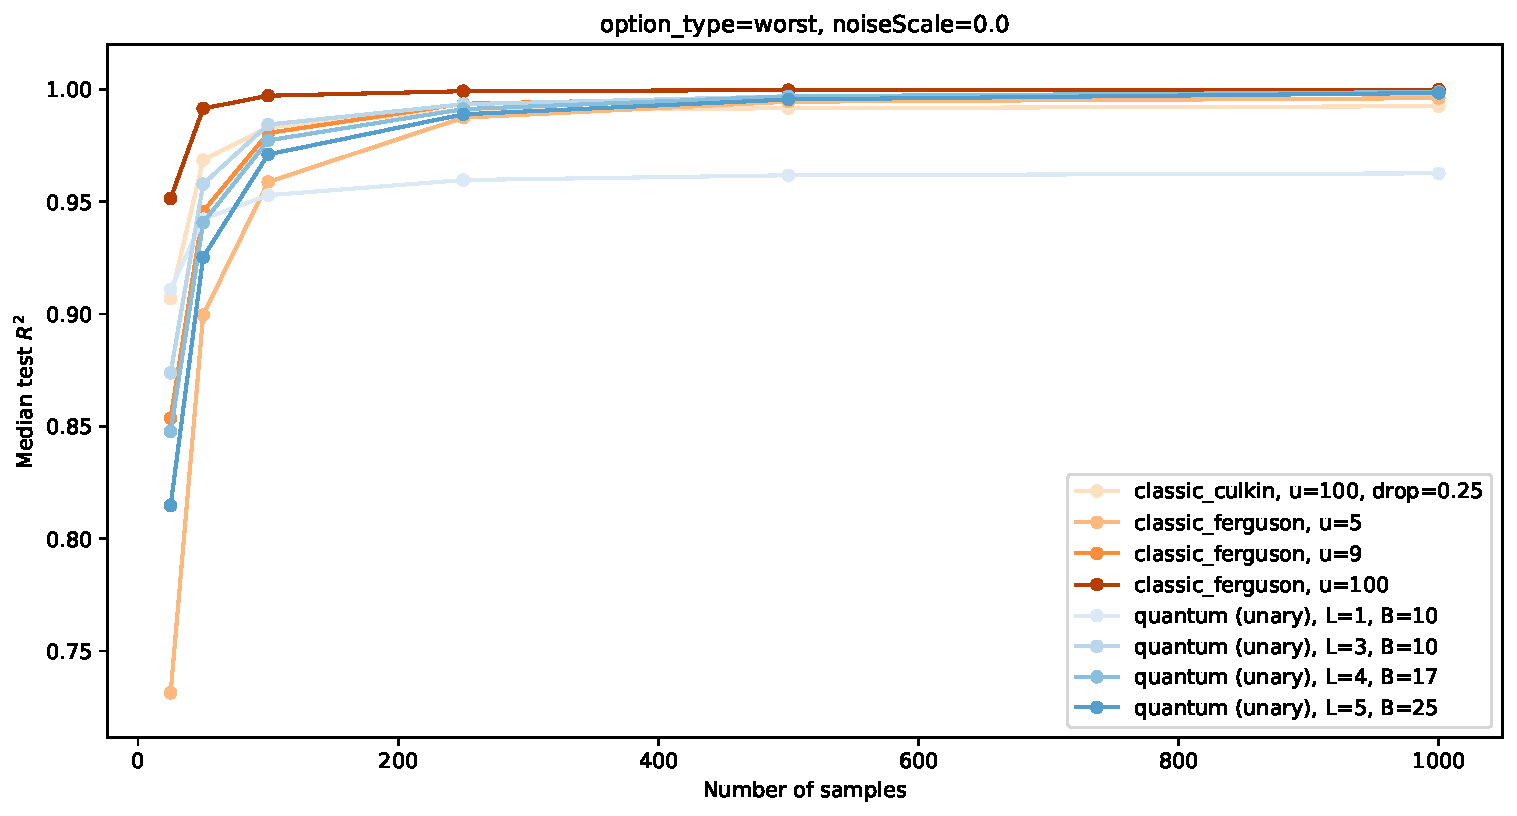
\includegraphics[width=\linewidth]{pictures/lineplot_samples0-1k_worst_nS0.pdf}
\caption{
Median test-$R^2$ as a function of the number of training observations
for the Worst-of payoff.
}
\label{fig:low_samples}
\end{figure}

Figure~\ref{fig:low_samples} shows the median test-$R^2$ for different
training dataset sizes.

For very small datasets ($N=25$), clear differences between the models
can be observed. For the classical Ferguson models, performance
increases with model size. The median $R^2$ rises from approximately
$0.73$ ($u=5$) to $0.85$ ($u=9$) and about $0.95$ ($u=100$).
The Culkin model also achieves solid results with about $0.91$,
thereby outperforming the smaller Ferguson variants.

For the quantum models, a different pattern emerges. Here, simpler
architectures appear to be more robust. The model with $L=1$ reaches
a median $R^2$ of approximately $0.91$ at $N=25$, whereas deeper
circuits perform worse ($L=3$: $\approx 0.87$, $L=4$: $\approx 0.85$,
$L=5$: $\approx 0.81$).

As the training dataset increases, the performance of all models
improves substantially. Already at $N=50$, several models achieve
$R^2$ values above $0.94$, and at $N=100$ most models exceed $0.97$.
In particular, the larger Ferguson models quickly achieve very high
accuracy; the model with $u=100$ reaches a median $R^2$ of about
$0.997$ already at $N=100$.

The VQC models also benefit from larger datasets. While shallower
architectures are more stable for small datasets, the deeper models
approach the performance of the classical networks as the amount
of training data increases. From approximately $N=250$ onwards,
the variants with $L=3$, $L=4$, and $L=5$ already reach $R^2$
values above $0.99$.

However, the simplest VQC model ($L=1$) scales more weakly.
Its median $R^2$ increases only from approximately $0.91$ at
$N=25$ to around $0.96$ at $N=1000$.

\section{Impact of Noise}
\label{sec:results-noise}

\begin{figure}[htbp]
\centering
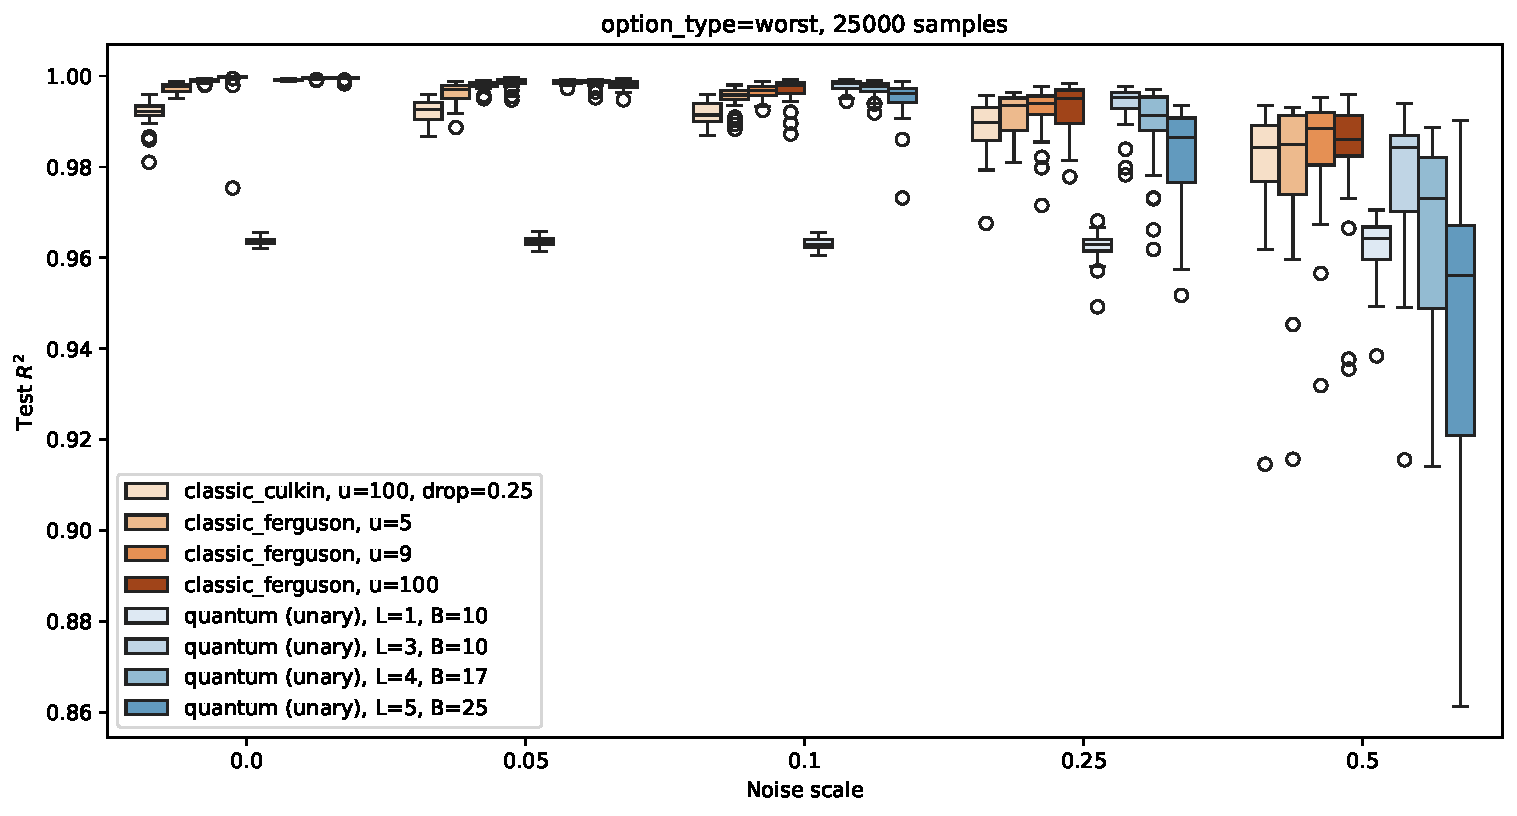
\includegraphics[width=\linewidth]{pictures/boxplot_noise_worst_25k.pdf}
\caption{
Distribution of test-$R^2$ values across 30 random initializations
for different noise intensities $\alpha$ for the Worst-of payoff
($N=25000$ training observations).
}
\label{fig:noise}
\end{figure}

Figure~\ref{fig:noise} shows the test-$R^2$ as a function of the
noise parameter $\alpha$ for the full training dataset.

At low noise intensities ($\alpha \le 0.1$), the performance of all
models remains close to the level of the baseline scenario. More
pronounced performance losses appear only at higher noise levels
($\alpha = 0.25$ and $0.5$).

The classical neural networks still achieve median values between
approximately $0.986$ and $0.988$ even at $\alpha = 0.5$. Larger
Ferguson architectures tend to show stronger absolute performance
declines. For example, the median for the largest model ($u=100$)
decreases from $0.99986$ in the baseline scenario to about $0.986$.

The Culkin model with dropout proves to be relatively robust. The
median test-$R^2$ decreases only from approximately $0.992$ to about
$0.984$, which can plausibly be attributed to the regularizing effect
of dropout.

For the VQC models, the sensitivity to noise strongly depends on the
circuit depth. The shallowest model ($L=1$) remains relatively stable
across all noise levels ($R^2 \approx 0.96$), although it already
achieves lower accuracy in the baseline scenario.

As the depth increases, the sensitivity to noise also increases.
While the model with $L=3$ still achieves about $0.984$ at
$\alpha = 0.5$, the median values for $L=4$ and $L=5$ drop to
approximately $0.973$ and $0.956$, respectively.

Overall, the results indicate that larger model capacity offers
advantages in the noise-free case but leads to stronger performance
degradation under increasing noise. Shallower models appear more
robust, although they are limited in their maximum approximation
capability.

\section{Combined Impact of Noise and Sample Size}
\label{sec:results-noise-samples}

\begin{figure}[htbp]
\centering
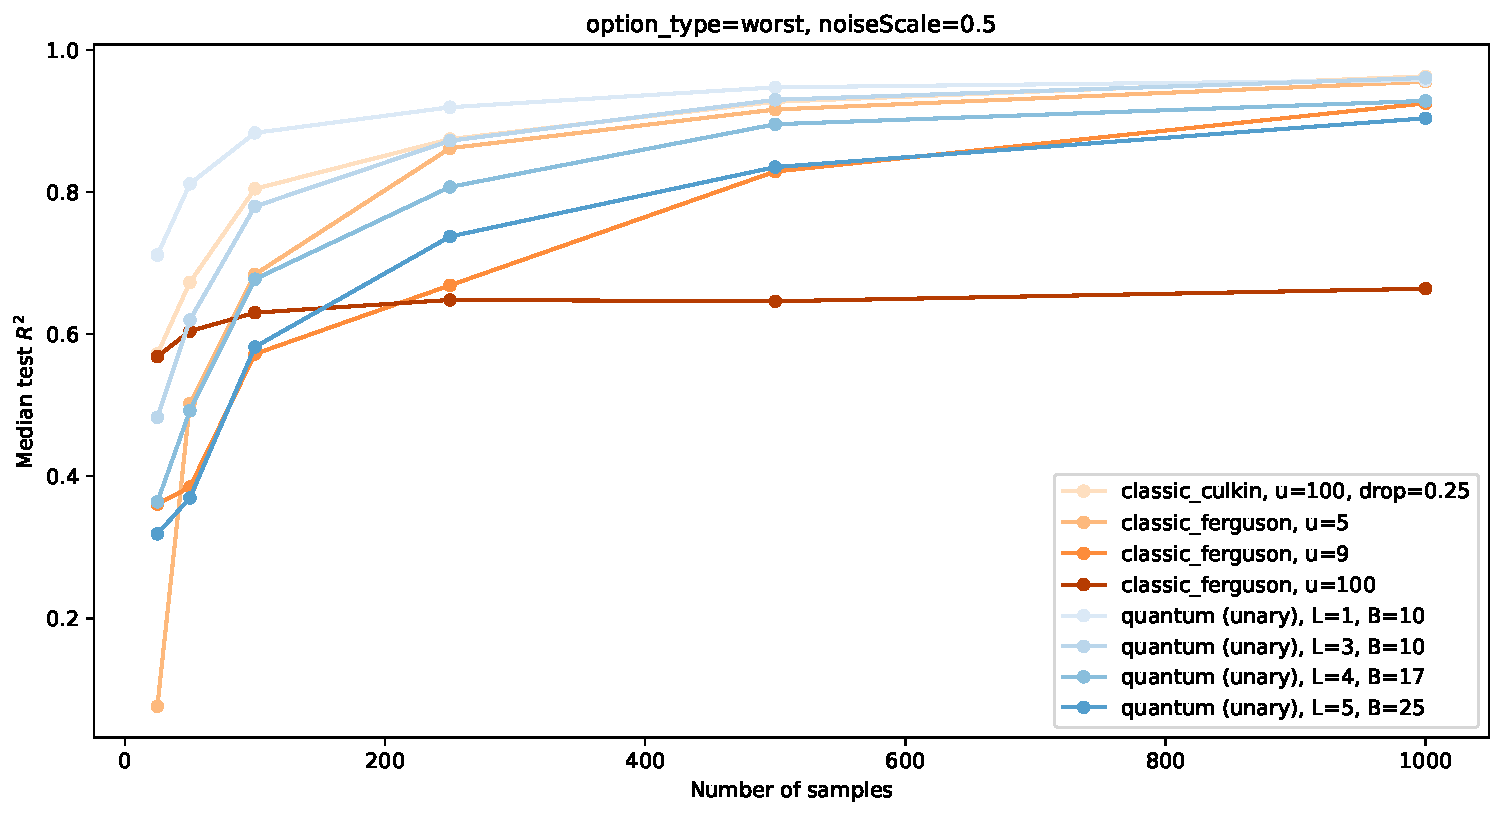
\includegraphics[width=\linewidth]{pictures/lineplot_samples0-1k_worst_nS05.pdf}
\caption{
Median test-$R^2$ as a function of training dataset size for the
Worst-of payoff under strong noise ($\alpha = 0.5$).
}
\label{fig:noise_samples}
\end{figure}

Figure~\ref{fig:noise_samples} shows the median test performance
for the combined scenario of strong training noise ($\alpha = 0.5$)
and varying training dataset size.

For very small datasets ($N=25$), the model architectures differ
substantially. The simplest VQC model ($L=1$) achieves the best
results with a median $R^2$ of about $0.71$, whereas deeper
variants perform considerably worse ($L=5$: $\approx 0.32$).

As the training dataset size increases, the deeper VQC models
improve substantially. At $N=1000$, the model with $L=1$ reaches
approximately $0.96$, while $L=3$ performs slightly better with
$R^2 \approx 0.961$. The models with $L=4$ and $L=5$ also benefit
strongly from larger datasets and reach approximately $0.93$
and $0.90$, respectively.

For the Ferguson architectures, a different pattern emerges.
At $N=25$, the largest model ($u=100$) achieves the best result
within this model family with about $0.57$, but still performs
considerably worse than the VQC model with $L=1$. The smallest
Ferguson model ($u=5$) performs particularly poorly with
$R^2 \approx 0.08$.

With increasing training dataset size, especially the smaller
Ferguson models improve substantially. The model with $u=5$
reaches a median $R^2$ of approximately $0.96$ at $N=1000$
and thus becomes one of the best-performing classical
architectures. In contrast, the largest Ferguson model
($u=100$) shows only limited improvement (from about $0.57$
to about $0.66$).

The Culkin model also benefits strongly from larger datasets.
Its median $R^2$ increases from about $0.57$ ($N=25$) to
approximately $0.96$ ($N=1000$), making it one of the best
performing classical models for larger datasets.

Overall, a clear trade-off between model capacity and data
availability can be observed. Simpler models are more robust
for very small datasets, whereas more complex architectures
reach their full potential only when sufficient training data
are available.


\section{Temporally Ordered Train-Test Split}
\label{sec:results-time-split}

\begin{figure}[htbp]
\centering
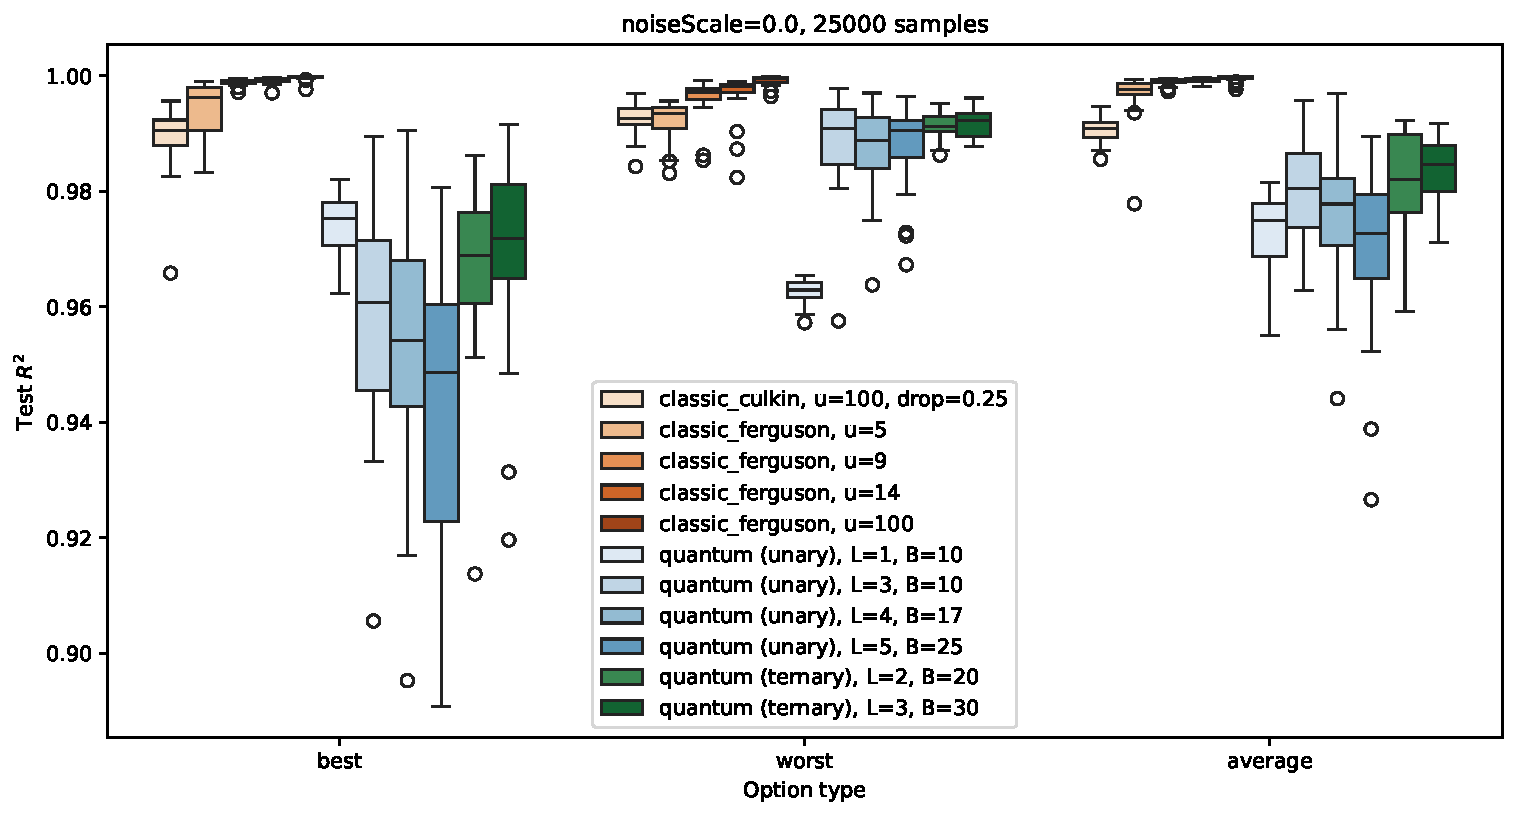
\includegraphics[width=\linewidth]{pictures/boxplot_optiontypes_nS0_nsp25k_time.pdf}
\caption{
Distribution of test-$R^2$ values across 30 seeds for Worst-of,
Best-of, and Average basket options in the baseline scenario with
a temporally ordered train–test split ($N=25000$, $\alpha=0$).
}
\label{fig:time_split}
\end{figure}

Figure~\ref{fig:time_split} shows the test-$R^2$ values for a temporally
ordered train–test split, in which only earlier observations are used
for training and later observations for testing.

The classical models largely retain their high predictive performance.
In particular, the larger Ferguson architectures continue to achieve
very high median values. For Average basket options, the median
test-$R^2$ increases from $0.9977$ ($u=5$) to $0.9991$ ($u=9$),
$0.9992$ ($u=14$), and $0.9997$ for the largest model ($u=100$).
The Culkin model performs slightly worse but still achieves high
values ($R^2 \approx 0.991$ for Average and $0.993$ for Worst-of).

In contrast, the VQC models show a noticeably stronger deterioration
compared to the random train–test split, particularly for the
Best-of payoff. Here, the median $R^2$ decreases with increasing
circuit depth from about $0.975$ ($L=1$) to $0.961$ ($L=3$),
$0.954$ ($L=4$), and $0.949$ ($L=5$).

Models with ternary encoding perform slightly better in this
scenario than the larger unary variants. For Best-of options,
they reach median values of approximately $0.969$ ($L=2$) and
$0.972$ ($L=3$).

For Worst-of options, the differences between the quantum models
are considerably smaller. The median values of the unary models
with $L=3$–$5$ lie between approximately $0.989$ and $0.991$,
while the ternary models reach similar values between
approximately $0.991$ and $0.992$.

Since the Best-of payoff is approximated significantly worse by
the quantum models under the temporally ordered split, this case
is examined in more detail. Figure~\ref{fig:error-analysis-timesplit-bestof}
shows the error structure in the Best-of scenario.

\begin{figure}[htbp]
\centering
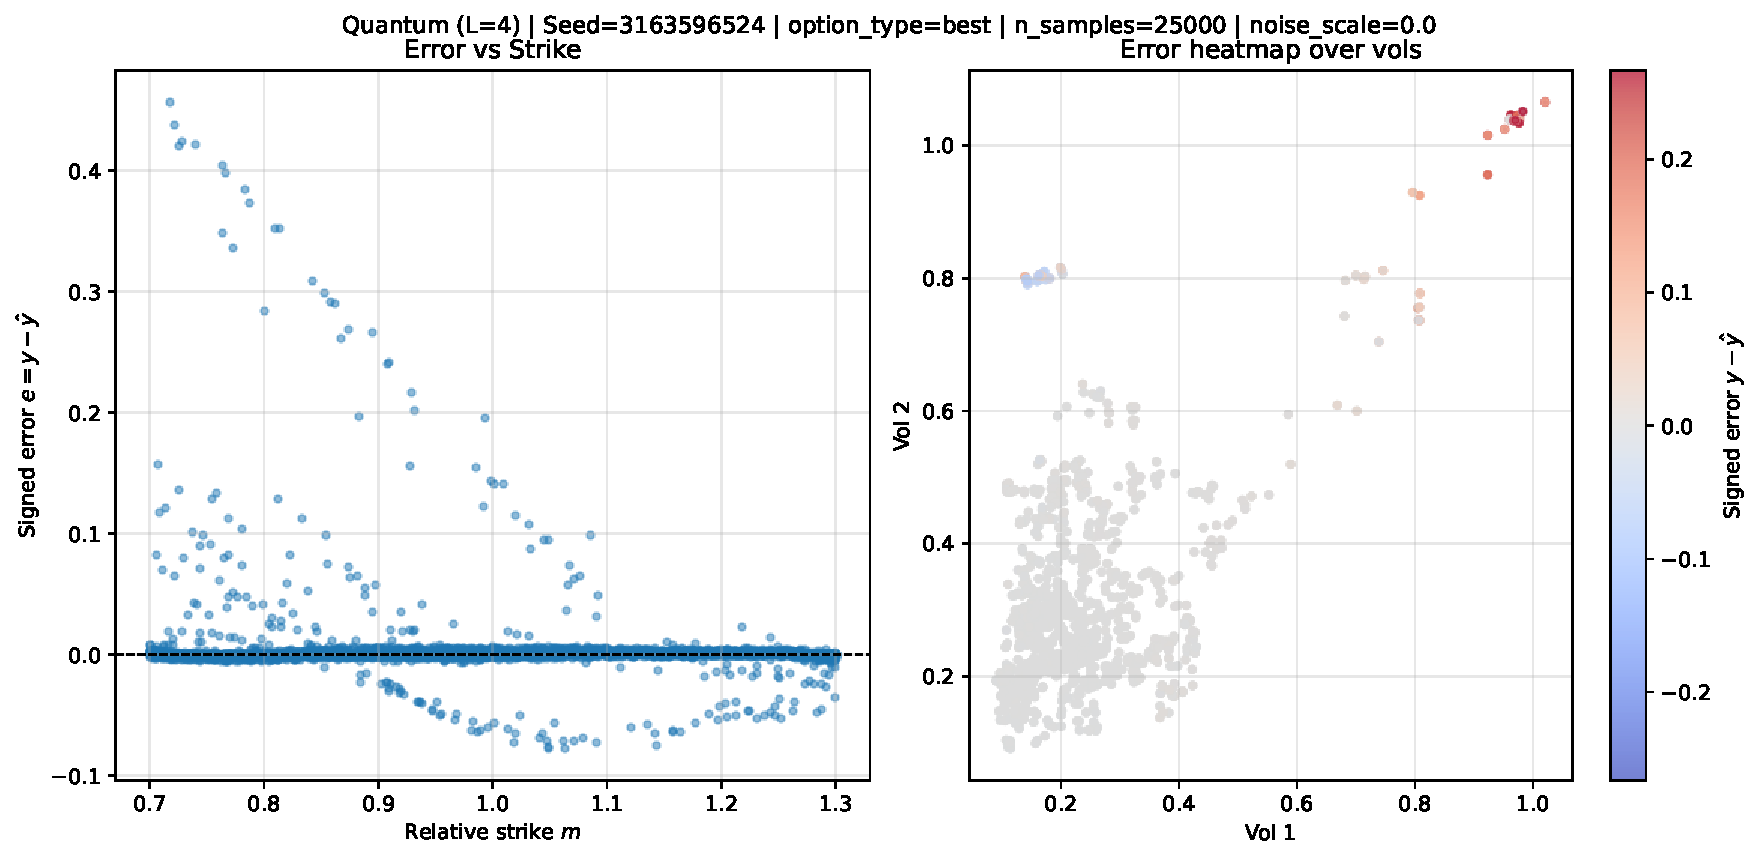
\includegraphics[width=\linewidth]{pictures/error_analysis_timesplit.pdf}
\caption{
Error analysis under the temporally ordered split (Best-of).
Left: error as a function of the relative strike.
Right: projection onto the volatility dimensions.
}
\label{fig:error-analysis-timesplit-bestof}
\end{figure}

Positive errors occur particularly for low strikes, corresponding
to a systematic underestimation of high option prices. In addition,
in contrast to the random train–test split, a clear concentration
of larger errors can be observed at simultaneously high volatility
levels.

Since a temporally ordered split is used, Figure~\ref{fig:vol-timesplit}
illustrates the temporal evolution of the rolling volatilities
together with the locations of the largest prediction errors.

\begin{figure}[htbp]
\centering
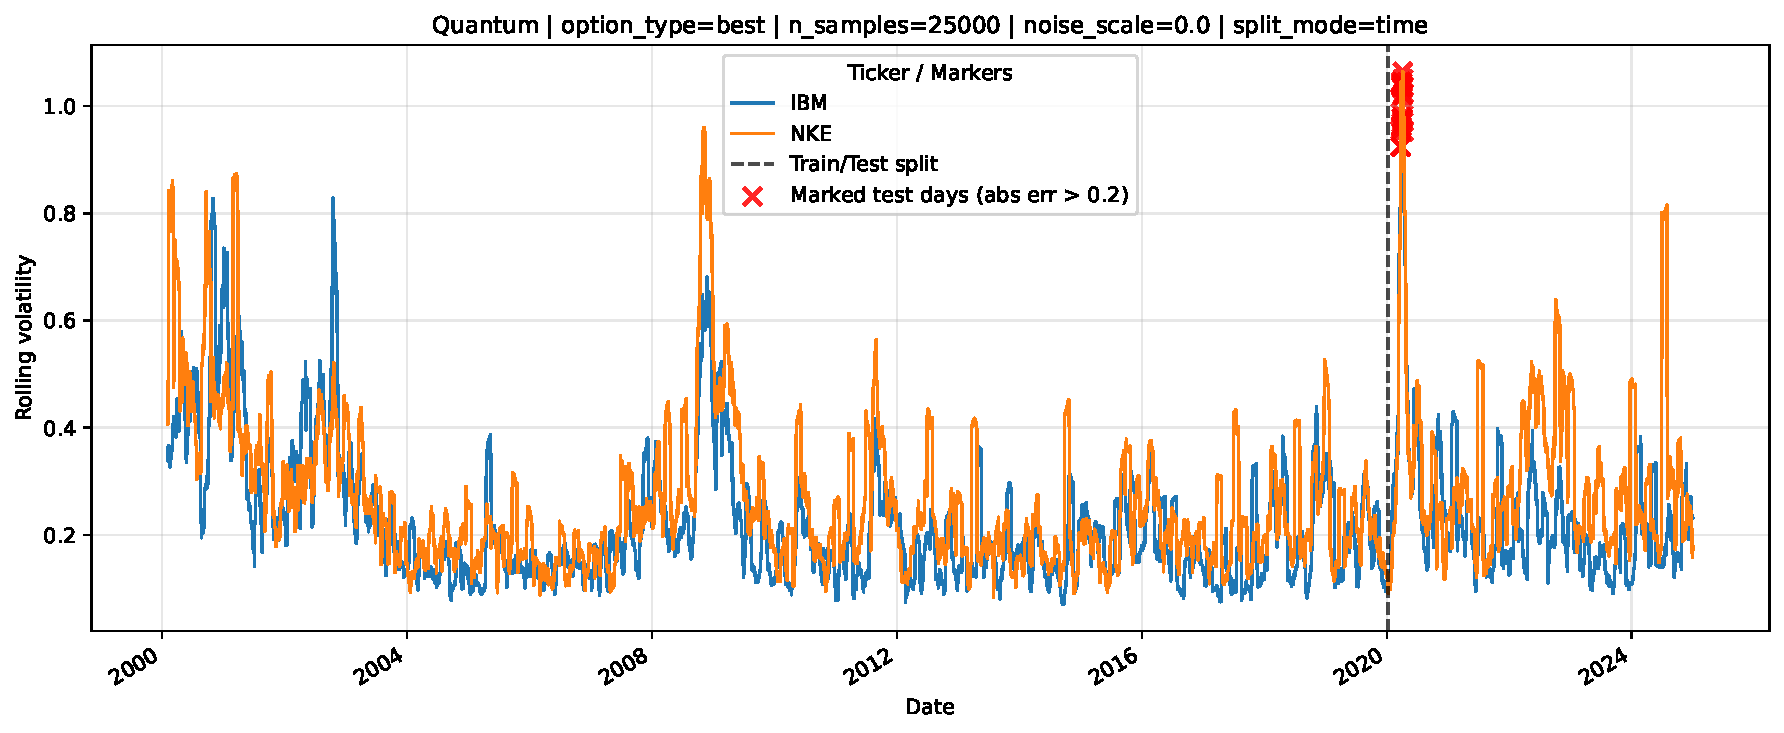
\includegraphics[width=\linewidth]{pictures/vol_timesplit_marked.pdf}
\caption{
Rolling volatilities with marked test days exhibiting large errors.
The dashed line indicates the boundary between the training and
test periods.
}
\label{fig:vol-timesplit}
\end{figure}

The highest volatility levels occur exclusively during the test
period. Large prediction errors concentrate in these phases,
while comparable volatility levels are not observed during the
training period. This indicates a distribution shift between
the training and test periods in the volatility features.